% CYBEL — IEEE ICRA 2027 submission. 8-page limit including references.
% Build: pdflatex main && bibtex main && pdflatex main && pdflatex main
\documentclass[conference]{IEEEtran}

\usepackage[T1]{fontenc}
\usepackage[utf8]{inputenc}
\usepackage{cite}
\usepackage{amsmath,amssymb}
\usepackage{graphicx}
\usepackage{booktabs}
\usepackage{url}
\usepackage{siunitx}
\usepackage{hyperref}
\usepackage{enumitem}
\usepackage{tikz}
\usepackage{pgfplots}
\pgfplotsset{compat=1.18}
\usetikzlibrary{arrows.meta,positioning,fit,calc}
\usepackage[section]{placeins}
\usepackage{stfloats}

\hypersetup{colorlinks=true,linkcolor=black,citecolor=black,urlcolor=black}
\sisetup{detect-all,range-phrase={--},range-units=single}

\newcommand{\ros}{\textsc{ros}}
\newcommand{\rosbridge}{\textsc{rosbridge}}
\newcommand{\rosapi}{\texttt{rosapi}}

\begin{document}

\title{Reclaiming Closed Service Robots: A Hypothesis-Driven
Methodology for Non-Destructive Protocol Reconstruction}

\author{
\IEEEauthorblockN{Claudia Lusamote Kimfuta}
\and
\IEEEauthorblockN{Sridath Tula}
}

\maketitle

\begin{abstract}
Commercial service robots are increasingly sold as closed Android--\ros{} systems: no public
SDK, no message schemas, and a vendor cloud that the owner cannot replace. A laboratory that
owns such a robot cannot modify its reception behaviour, and cannot even establish which
commands the machine accepts. We present a non-destructive methodology for recovering that
command surface without vendor cooperation, structured as four falsifiable hypotheses about
where the protocol is observable and how to verify it, tested through a seven-phase pipeline
that triangulates network mapping, \rosapi{} introspection, static analysis of the vendor
application, and passive broker observation. We validate the methodology on a commercially
available reception robot, recovering \num{455} topics and \num{308} services and
rebuilding teleoperation, navigation, speech and visitor interaction as an edge platform that
runs without the vendor cloud. Our main empirical finding concerns verification rather than
discovery. A transport-level acknowledgment says nothing about whether the machine moved. In
\num{17} logged field commands, what separated success from failure was the localization state
the robot reported: all ten failures occurred while it reported itself unlocalized, and all
seven successes while it reported navigating. How the goal was addressed made no difference at
all. A controlled bench comparison shows the same asymmetry between an unprepared and a
prepared command path. We report field indicators with confidence intervals, a capability
comparison against the vendor application, and the conditions under which each hypothesis
should transfer to other closed platforms.
\end{abstract}

\begin{IEEEkeywords}
Service robotics, reverse engineering, vendor lock-in, \rosbridge{}, edge computing
\end{IEEEkeywords}

%==============================================================================
\section{Introduction}
\label{sec:intro}
%==============================================================================

A laboratory that buys a commercial service robot buys a sealed appliance. The vendor ships an
Android application, a cloud account, and a support contract; it does not ship the message
schemas that would let the owner send the robot anywhere the application does not already go.
For research groups this is a hard limit: the platform in Fig.~\ref{fig:robot} navigates,
speaks and greets visitors perfectly well, but only in the ways its manufacturer anticipated.

\begin{figure}[!t]
\centering
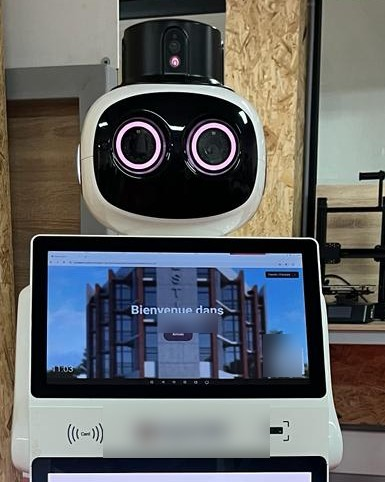
\includegraphics[width=0.62\columnwidth]{fig/robot_kiosk}
\caption{The study platform running our reconstructed visitor interface on its own touchscreen.
The head is an Android computer; the mobile base underneath is a separate Linux/\ros{} machine.
Neither exposes a documented interface to its owner. Identifying marks are blurred.}
\label{fig:robot}
\end{figure}

\textbf{Why this is hard.} Three obstacles compound, and none of them is peculiar to this
vendor. First, the robot is not one computer but two: an Android head and a \ros{} chassis,
joined by an undocumented internal link. No single point of observation covers the whole command
surface, and each one is blind in a different place (Section~\ref{sec:method}). Second, there is
no white-box route. Shells on the chassis are closed, and repeated authentication attempts lock
the account, so we cannot simply read the running system. Third, and least obvious, the software
layer that accepts a message is not the layer that turns the wheels. A command can be accepted,
acknowledged and then quietly dropped. Treat the acknowledgment as proof and the result is a
protocol description that is confidently wrong. This is the reason naive fuzzing of the exposed
interfaces gets nowhere on such a platform.

\textbf{Research question.} \emph{Can a non-destructive methodology recover the command surface
of a closed Android--\ros{} robot without documentation, and what evidence is required before a
recovered command may be considered validated?}

We formulate four hypotheses, stated here and resolved in Section~\ref{sec:eval}:

\begin{itemize}[leftmargin=1.2em]
\item \textbf{H1 (application-as-specification).} Static analysis of the vendor's own Android
application yields the wire protocol the chassis actually speaks.
\item \textbf{H2 (broker-as-command-channel).} The exposed MQTT broker can issue motion
commands, as the WebSocket bridge does.
\item \textbf{H3 (map-artifact reuse).} Reusing the vendor's own map annotations is more
reliable than re-deriving goal coordinates offline.
\item \textbf{H4 (transport $\neq$ execution).} A transport acknowledgment does not imply that
the chassis executed the command.
\end{itemize}

\textbf{Contributions.}
\begin{enumerate}[label=\textbf{C\arabic*.},leftmargin=1.5em]
\item A reproducible seven-phase reverse-engineering methodology for closed Android--\ros{}
robots, organised around falsifiable hypotheses and a triangulation rule, together with the
effort it required in practice (Sections~\ref{sec:method} and~\ref{sec:eval}).
\item A recovered command surface for a commercial reception platform and an edge-first
architecture built on it, including a speech channel obtained through Android inter-process
communication after every protocol-level channel had been eliminated
(Section~\ref{sec:platform}).
\item Field evidence that execution must be verified against state telemetry rather than
transport acknowledgments, with the resulting design rule, quantified indicators, and an
analysis of which findings should transfer to other closed platforms
(Sections~\ref{sec:eval} and~\ref{sec:discussion}).
\end{enumerate}

All work reported here was carried out on hardware owned by our institution, for
interoperability purposes, without redistributing vendor code or circumventing any licensing
mechanism; Section~\ref{sec:discussion} details the ethical and legal framing.

%==============================================================================
\section{Related Work}
\label{sec:related}
%==============================================================================

\subsection{Re-engineering commercial robot platforms}
The closest precedent is Kim \emph{et al.}~\cite{kim2005reengineering}, who re-engineered the
software architecture of a commercial home service robot. Their study follows much the same arc
as ours, but one difference decides everything: they had the manufacturer's source code and its
engineering team, while we start from a sealed product. M\"uhe \emph{et al.}~\cite{muhe2010kuka}
recovered a proprietary industrial robot language, again working from artifacts the vendor had
published. Both begin with more material than we do, and the methodology below exists mainly to
make up for that shortfall.

\subsection{Vendor lock-in and interoperability}
The trade-off between proprietary and open platform strategies is long
established~\cite{west2003open}, and service robotics reproduces it one product at a time.
Glauser \emph{et al.}~\cite{glauser2023interop} report healthcare deployments held back by
outdated and restrictive vendor SDKs, and propose an interoperable programming interface as the
remedy. Middleware bridges such as ROS--YARP~\cite{aragao2016yarp} address the adjacent problem
of connecting two interfaces that are both \emph{known}. In every case the interface itself is
taken for granted. The question we take up comes earlier: how does a laboratory obtain one at
all, on a robot it has already bought?

\subsection{Black-box access to \ros{} systems}
\rosbridge{} was designed to let non-\ros{} clients reach a \ros{} graph over
WebSocket~\cite{crick2012rosbridge,rosbridge_suite}, normally deployed by the integrator who
controls that graph. DeMarinis \emph{et al.}~\cite{demarinis2019scanning} inverted this
perspective, scanning the Internet for exposed \ros{} systems and showing that sensors and
actuators can be reached without any knowledge of the node graph; Dieber \emph{et
al.}~\cite{dieber2017security} treat the same openness as an application-level security problem.
We occupy a similar position with the sign reversed: we too arrive at a vendor-deployed bridge
as an unknown client, but constructively, and on hardware we own.

\subsection{Protocol recovery from companion software}
Extracting protocol specifications from observed traffic is a mature security
technique~\cite{comparetti2009prospex}, and Android analysis has focused on information flow
within an application~\cite{enck2014taintdroid} or between applications~\cite{chin2011android}.
The practice of reading a device's companion app to recover its wire protocol is established in
the IoT community~\cite{giese2018xiaomi}. Hypothesis H1 imports that practice into robotics,
where the companion application controls a second, physically separate computer.

\subsection{Edge robotics and on-device interaction}
Cloud robotics assumes a reliable path to remote compute~\cite{kehoe2015cloud}. We had the
opposite constraint. The robot's own network guarantees no Internet route, so speech and
recognition had to run on the head, which pushed us towards closed-vocabulary
recognition~\cite{warden2018speechcommands,vosk} and on-device face
embeddings~\cite{schroff2015facenet}. Language-model agents~\cite{ahn2022saycan,driess2023paleme}
assume an open action API is already available. On a closed robot that API has to be recovered
first, which is the work reported here.

\begin{table}[!t]
\caption{Positioning relative to the nearest categories of work}
\label{tab:positioning}
\centering
\scriptsize
\setlength{\tabcolsep}{3pt}
\begin{tabular}{@{}p{1.55cm}p{2.5cm}p{3.0cm}@{}}
\toprule
\textbf{Work} & \textbf{Primary emphasis} & \textbf{Distinction in this paper} \\
\midrule
Kim \emph{et al.}~\cite{kim2005reengineering} & Re-architecting a service robot &
Vendor source and engineers available; here the product is sealed \\[2pt]
M\"uhe \emph{et al.}~\cite{muhe2010kuka} & Proprietary robot language &
Published artifacts as input; here no artifact is published \\[2pt]
DeMarinis \emph{et al.}~\cite{demarinis2019scanning} & Exposed \ros{} systems at scale &
Same black-box stance, applied constructively to one owned unit \\[2pt]
Glauser \emph{et al.}~\cite{glauser2023interop} & Interoperable interface for social robots &
Assumes a usable SDK; we recover one where none exists \\[2pt]
Giese \emph{et al.}~\cite{giese2018xiaomi} & Companion-app protocol recovery (IoT) &
Transposed to a robot whose app drives a separate \ros{} computer \\[2pt]
\textbf{This work} & \textbf{Non-destructive protocol reconstruction} &
\textbf{Hypothesis-driven method; execution verified against state, not transport} \\
\bottomrule
\end{tabular}
\end{table}

Table~\ref{tab:positioning} sets out the gap. Each neighbouring line of work starts once the
interface is known; what we describe here is the step before that.

%==============================================================================
\section{Platform and Access Model}
\label{sec:access}
%==============================================================================

The study platform is a mass-produced indoor reception robot, sold as a turnkey product with a
companion Android application and a subscription cloud service. It pairs a Linux/\ros{}
chassis~\cite{quigley2009ros} carrying SLAM, a planner, LiDAR and RGB-D sensing with an
Android~7.1 head that drives a \SI{15.6}{inch} touchscreen, cameras and speakers. We refer to it
generically throughout, since nothing in the methodology depends on the particular model and we
have no interest in singling out one manufacturer. The two computers run independent network
stacks, a fact no vendor document states and no application string reveals.

\begin{figure}[!t]
\centering
\resizebox{0.95\columnwidth}{!}{%
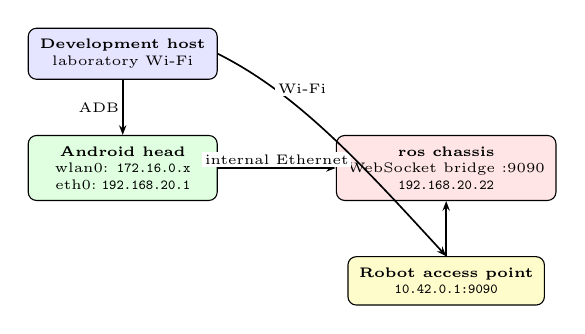
\begin{tikzpicture}[
  node distance=0.7cm and 1.5cm,
  box/.style={draw, rounded corners=3pt, align=center, font=\tiny,
              inner sep=4pt, minimum width=2.4cm},
  arr/.style={-{Stealth[length=3.5pt]}, semithick},
  lbl/.style={font=\tiny, fill=white, inner sep=1pt}
]
  \node[box, fill=blue!10] (pc) {\textbf{Development host}\\laboratory Wi-Fi};
  \node[box, fill=green!12, below=0.7cm of pc] (head)
    {\textbf{Android head}\\wlan0: \texttt{172.16.0.x}\\eth0:\;\texttt{192.168.20.1}};
  \node[box, fill=red!10, right=1.5cm of head] (ch)
    {\textbf{\ros{} chassis}\\WebSocket bridge :9090\\\texttt{192.168.20.22}};
  \node[box, fill=yellow!20, below=0.7cm of ch] (ap)
    {\textbf{Robot access point}\\\texttt{10.42.0.1:9090}};
  \draw[arr] (pc)   -- node[lbl, left]{ADB} (head);
  \draw[arr] (head) -- node[lbl, above]{internal Ethernet} (ch);
  \draw[arr] (pc.east) .. controls +(1.0,-0.5) and +(-1.1,1.2) ..
             node[lbl, near start, right]{Wi-Fi} (ap.north);
  \draw[arr] (ap)   -- (ch);
\end{tikzpicture}%
}
\caption{Three network segments on a product marketed as a single device. Conflating the head's
DHCP address with the chassis address was the most frequent operator error we observed.}
\label{fig:network}
\end{figure}

Network mapping turned up three segments (Fig.~\ref{fig:network}), and that was already a
result in itself. Two channels are reachable from outside the vendor stack: a WebSocket bridge
on port~9090 and an MQTT broker on port~1883. Shell access to the chassis is closed. We observed
that repeated authentication attempts trigger an account lockout, and went no further down that
road, partly because it would break the non-destructive principle stated below and partly
because we had one unit and bricking it would have ended the study. Two vendor packages sit on
the head, a welcome application and a deployment tool, and both link against the same
chassis-communication library. We treat that library as the \emph{de facto} protocol
specification. It is the empirical basis for H1.

%==============================================================================
\section{Methodology}
\label{sec:method}
%==============================================================================

\subsection{Principles}

Four rules govern the procedure. \textbf{P1: observe before publishing.} We listen passively
before injecting anything, because there is no way to predict how an undocumented
safety-critical system will react. \textbf{P2: verify effects, not acknowledgments.} A command
counts as validated only once an independent state topic changes. This is the working form of
H4. \textbf{P3: triangulate.} We accept a finding only when two independent sources agree, drawn
from network traces, introspection, decompiled application code and field logs. \textbf{P4:
remain non-destructive.} No firmware modification, no root, no persistent change to vendor
partitions. This is an ethical commitment, and with a single unit it is also what makes the
work repeatable.

\subsection{Vantage points and their blind spots}

The whole methodology exists because no single observation point tells us enough
(Fig.~\ref{fig:vantage}). Introspection lists names, but says nothing about preconditions.
Traffic capture shows what the vendor application happened to send during one session, which is
not the same as what the chassis would accept. Decompiled code gives intent and the implicit
setup steps, but leaves open whether a given path is reachable on this firmware. Triangulating
between the three is not a stylistic preference; it is the only way to cover what any one of
them misses.

\begin{figure}[!t]
\centering
\resizebox{0.95\columnwidth}{!}{%
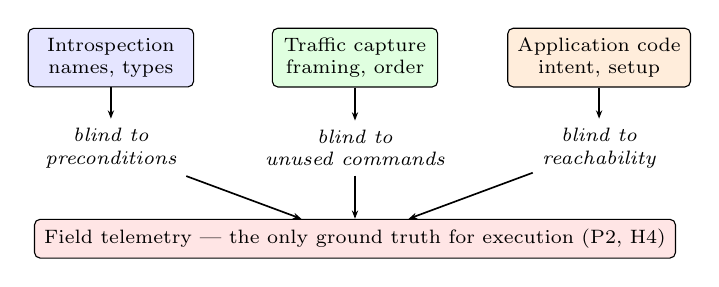
\begin{tikzpicture}[
  vp/.style={draw, rounded corners=2pt, align=center, font=\scriptsize,
             inner sep=3.5pt, minimum width=2.1cm},
  gap/.style={font=\scriptsize\itshape, align=center},
  arr/.style={-{Stealth[length=3pt]}, semithick}
]
  \node[vp, fill=blue!10]   (a) at (0,0)      {Introspection\\\scriptsize names, types};
  \node[vp, fill=green!12]  (b) at (3.1,0)    {Traffic capture\\\scriptsize framing, order};
  \node[vp, fill=orange!14] (c) at (6.2,0)    {Application code\\\scriptsize intent, setup};
  \node[gap] (a2) at (0,-1.15)   {blind to\\preconditions};
  \node[gap] (b2) at (3.1,-1.15) {blind to\\unused commands};
  \node[gap] (c2) at (6.2,-1.15) {blind to\\reachability};
  \draw[arr] (a)--(a2); \draw[arr] (b)--(b2); \draw[arr] (c)--(c2);
  \node[vp, fill=red!10, minimum width=6.2cm] (t) at (3.1,-2.3)
    {Field telemetry --- the only ground truth for execution (P2, H4)};
  \draw[arr] (a2)--(t); \draw[arr] (b2)--(t); \draw[arr] (c2)--(t);
\end{tikzpicture}%
}
\caption{Each vantage point answers a different question and is blind to the others. A
recovered command is accepted only after state telemetry confirms a physical effect.}
\label{fig:vantage}
\end{figure}

\subsection{The seven-phase pipeline}

Table~\ref{tab:phases} gives, for each phase, the evidence it produces, the hypothesis it bears
on, and the condition under which we stopped. The stopping criteria are not a formality. With
455 topics on the wire, an exploration without them simply does not converge.

\begin{table}[!t]
\caption{Reverse-engineering pipeline}
\label{tab:phases}
\centering
\scriptsize
\setlength{\tabcolsep}{3pt}
\begin{tabular}{@{}p{0.15cm}p{1.25cm}p{2.35cm}p{0.5cm}p{2.15cm}@{}}
\toprule
\textbf{\#} & \textbf{Phase} & \textbf{Evidence produced} & \textbf{Hyp.} & \textbf{Stopping criterion} \\
\midrule
1 & Network mapping & Segment map, open ports & --- & All hosts and reachable ports enumerated \\
2 & Introspection & Topic and service inventory & H1 & Inventory stable across sessions \\
3 & Passive broker & Payload classes on the broker & H2 & No command payload after repeated sessions \\
4 & Application audit & Names, types, implicit setup steps & H1 & Every observed name located in code \\
5 & Frame capture & Message framing and ordering & H1 & Client reproduces vendor framing \\
6 & Edge integration & On-device services and bridges & --- & Capability reachable without a host PC \\
7 & Field validation & State transitions, pose deltas & H3, H4 & Effect confirmed on independent topic \\
\bottomrule
\end{tabular}
\end{table}

We kept the negative results instead of discarding them: a legacy velocity topic with no
subscriber, two candidate speech topics, three HTTP ports on the head, and the broker command
path of H2. Each one closed a branch of the search, which is worth as much as an open one.

Phases~1--6 took two weeks and phase~7 a further week, spread over eight sessions with the
physical robot and carried out by one full-time engineer. We decompiled two applications;
introspection returned \num{455} topics and \num{308} services. The exploration scripts, the
recovered interface description and the logs behind every figure and table below are archived
and released with this paper~\cite{cybel2026}, so that the pipeline can be replayed elsewhere.

%==============================================================================
\section{Recovered Command Surface and Edge Platform}
\label{sec:platform}
%==============================================================================

\subsection{Command and telemetry}

Motion is commanded by advertising a multiplexer input and then publishing twist messages on it
at roughly \SI{10}{\hertz}. The vendor application quietly sets a manual-control mode when a
session opens. Our early builds did not, and every command we sent was dropped without comment.
That precondition was visible in the decompiled application and in no traffic capture we took,
and it was our first concrete encounter with H4. Autonomous motion comes in two forms: a
coordinate goal, and a named-annotation service backed by the vendor's marker manager. One
status field reports the state machine gating both, with values for unlocalized, ready,
navigating, arrived and error. We throttle subscriptions per topic to keep the bridge usable
over the robot's Wi-Fi.

One detail cost us time and is worth passing on. A single vendor message type, carrying one
integer field, is reused across several unrelated services, each giving that integer its own
private meaning. Call one of them with empty or guessed arguments and it returns success, then
either does nothing or does the opposite of what was intended. We recovered the correct
arguments through the same introspection route that supports H1. Interfaces reconstructed from
the outside are prone to this, and an acknowledgment offers no protection against it.

\subsection{Edge architecture}

The reconstructed platform is edge-first by necessity, since the robot's network offers no
guaranteed Internet path. A domain layer hides the robot behind one interface with two
implementations, simulated and real. This let us exercise the logic under 169 unit tests without
the physical machine, and it kept ordinary software defects separate from genuine protocol
uncertainty, which during field sessions was the difference between a productive afternoon and a
wasted one. Above it, an application layer exposes REST and WebSocket endpoints and runs either
on a development machine or on the Android head, so a visitor session needs no external
computer. A presentation layer serves the visitor interface of Fig.~\ref{fig:robot} and the
operator console.

\subsection{Speech through inter-process communication}

Speech was the hardest capability to recover, and at the protocol level the search simply
failed. No topic accepted text, no such service existed, the head's HTTP ports were closed, and
the broker carried telemetry only. The reason turned out to be architectural rather than
accidental. The vendor implements speech inside the Android application layer, over opaque IPC
to a bundled engine, so it was never a robot-level capability at all and no amount of protocol
search would have found it. The answer was to stop looking sideways and move up a layer. A
\SI{50}{\kilo\byte} companion application registers a broadcast
receiver~\cite{chin2011android} and hands incoming text to the platform's native speech engine:

\begin{footnotesize}
\begin{verbatim}
am broadcast -n com.cybel.ttsbridge/.SpeakReceiver
  -a com.cybel.ttsbridge.SPEAK --es text "Welcome."
\end{verbatim}
\end{footnotesize}

\noindent The move itself generalises. Whenever a vendor implements a function in the
application layer, no protocol-level search will reach it, and the host operating system is
where the capability has to be picked up instead.

\subsection{Interaction layer}

Visitor interaction runs entirely on the head. We abandoned free dictation early: a compact
offline model holds no pronunciation for the proper nouns that matter on a campus, and it
transcribed them unreliably in front of visitors. Recognition now works from a closed vocabulary
rebuilt at request time out of the deployed annotations and the question set. The same
limitation caught us again with the wake phrase. Built from the platform's invented name, it was
consistently decoded as an unrelated word the model did in fact know; replacing it with a
phonetically close phrase made of real words solved the problem. Face re-identification runs on
the head at roughly \SI{1}{\hertz} and sends only embedding vectors, never images.

%==============================================================================
\section{Experimental Evaluation}
\label{sec:eval}
%==============================================================================

Our samples are small, so we give proportions with Wilson score
intervals~\cite{wilson1927,brown2001interval}, which stay well behaved at these sizes, and we
state every trial count.

\subsection{H1 confirmed, H2 rejected}

Every topic and service name we later exercised on the wire had first been found in the
decompiled vendor library, and so had preconditions like the manual-mode gate that no traffic
capture ever showed us. There is a structural reason for this. The vendor's own application has
to speak the real protocol in order to drive the chassis, so its compiled code is a lower bound
on the command surface in a way that documentation, which may describe intentions rather than
behaviour, is not. We did not test the converse. Whether commands exist that the application
never uses remains open, and Section~\ref{sec:discussion} records it as a limitation.

H2 is rejected. Wildcard subscription across several sessions returned one telemetry topic
carrying odometry, and no payload we replayed changed the robot's state. The vendor library
explains the result: its broker client is wired only to telemetry publishers, and the command
path runs exclusively over the WebSocket bridge. On this platform the broker cannot carry
commands at all. We report the rejection because MQTT is a reasonable first guess for anyone
approaching a machine like this, and rediscovering that it leads nowhere is expensive.

\subsection{H4: transport acknowledgment is not execution}

\begin{figure}[!t]
\centering
\resizebox{\columnwidth}{!}{%
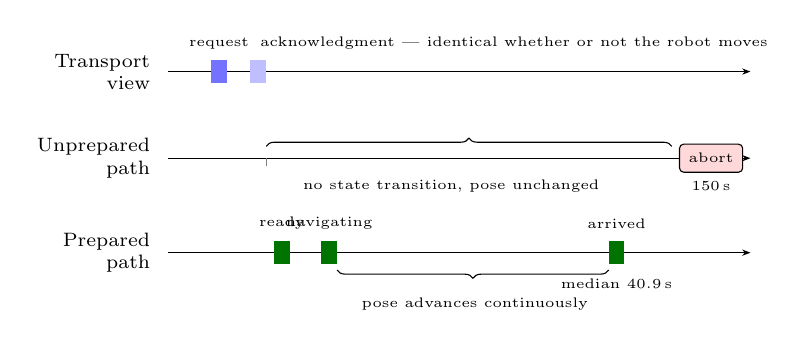
\begin{tikzpicture}[font=\scriptsize, >={Stealth[length=3pt]}]
  \def\L{7.4}
  % lane A : transport
  \draw[->] (0,2.2) -- (\L,2.2) node[right]{};
  \node[left, align=right] at (-0.1,2.2) {Transport\\view};
  \fill[blue!55] (0.55,2.05) rectangle (0.75,2.35);
  \node[above, font=\tiny] at (0.65,2.36) {request};
  \fill[blue!25] (1.05,2.05) rectangle (1.25,2.35);
  \node[above right, font=\tiny] at (1.05,2.36)
    {acknowledgment --- identical whether or not the robot moves};
  % lane B : unprepared
  \draw[->] (0,1.1) -- (\L,1.1);
  \node[left, align=right] at (-0.1,1.1) {Unprepared\\path};
  \draw[dashed, gray] (1.25,1.0) -- (1.25,1.2);
  \node[font=\tiny, align=center] at (3.6,0.75) {no state transition, pose unchanged};
  \draw[decorate, decoration={brace, amplitude=3pt}] (1.25,1.25) -- (6.4,1.25);
  \node[draw, fill=red!15, rounded corners=1.5pt, font=\tiny] at (6.9,1.1) {abort};
  \node[font=\tiny] at (6.9,0.75) {\SI{150}{\second}};
  % lane C : prepared
  \draw[->] (0,-0.1) -- (\L,-0.1);
  \node[left, align=right] at (-0.1,-0.1) {Prepared\\path};
  \fill[green!45!black] (1.35,-0.25) rectangle (1.55,0.05);
  \node[above, font=\tiny] at (1.45,0.08) {ready};
  \fill[green!45!black] (1.95,-0.25) rectangle (2.15,0.05);
  \node[above, font=\tiny] at (2.05,0.08) {navigating};
  \fill[green!45!black] (5.6,-0.25) rectangle (5.8,0.05);
  \node[above, font=\tiny] at (5.7,0.08) {arrived};
  \node[font=\tiny] at (5.7,-0.5) {median \SI{40.9}{\second}};
  \draw[decorate, decoration={brace, mirror, amplitude=3pt}] (2.15,-0.32) -- (5.6,-0.32);
  \node[font=\tiny] at (3.9,-0.75) {pose advances continuously};
\end{tikzpicture}%
}
\caption{The transport lane is identical whether or not the command executes. Only an
independent state topic distinguishes the two lower cases. Timings from the bench comparison of
Section~\ref{sec:eval}-C ($n=3$ per arm).}
\label{fig:h4}
\end{figure}

The bridge acknowledges any syntactically valid message it can route to a subscriber. That
acknowledgment is produced above the chassis safety and mode-arbitration layer, which means it
certifies the first hop and nothing beyond it (Fig.~\ref{fig:h4}). Our field record shows what
this costs in practice. Across \num{17} logged navigation commands, the outcome followed the
reported localization state exactly: all ten failures happened while the robot reported itself
unlocalized, all seven successes while it reported navigating. The same split holds for both
goal-addressing schemes, coordinate goals failing five times and succeeding once, named
annotations failing five times and succeeding six. In this record the addressing scheme explains
nothing and the precondition state explains everything. Every one of the failed commands had
been acknowledged.

\subsection{H3: addressing scheme versus preparation}

\begin{figure}[!t]
\centering

\includegraphics[width=\columnwidth]{fig/vendor_map}
\caption{The vendor deployment application showing the \SI{1235}{\meter\squared} laboratory map
used throughout this study, with its annotated points of interest. These annotations live in the
chassis marker manager; reusing them avoids the drift that affects coordinates extracted
offline, but does not by itself make navigation succeed (Section~\ref{sec:eval}-C).}
\label{fig:vendormap}
\end{figure}

Goal annotations are created in the vendor deployment application (Fig.~\ref{fig:vendormap})
and resolved by the chassis marker manager. We compared the two schemes directly on the bench,
with automatic mode set and telemetry subscribed for both arms, navigating to the same annotated
target
(Fig.~\ref{fig:results}\,(a)). Coordinate goals succeeded in 3 of 3 trials, reaching the
arrived state in \SIlist{40.0;40.9;46.5}{\second} (median \SI{40.9}{\second}). The annotation
service, issued from the same bare client through its full fallback chain, produced no state
transition at all in 3 of 3 trials and was abandoned at the \SI{150}{\second} timeout. At three
trials per arm the difference is not statistically significant (Fisher's exact test, two-sided,
$p=0.10$), and neither arm's interval excludes the other's point estimate.

Taken alone this would be a clean verdict against annotation reuse, and it would also contradict
everything we saw in daily operation, where the annotation route is precisely the one that
works. Three consecutive guided tours ran to completion without operator intervention, 30
navigation legs in total counting nine resolvable stops and a return leg per tour, with
durations of \SIlist{667.6;670.4;822.3}{\second}. What reconciles the two observations is
everything the bare client leaves out. The operational path checks control state, clears
blocking navigation states, relocalizes when the robot reports itself unlocalized or below the
\SI{60}{\percent} confidence gate, and declines to issue a goal if those conditions are not met.
The bare client does none of this and fires into the void.

We therefore do not claim H3 in the form we stated it. What the evidence supports is broader and
more useful: what decides the outcome is not how the goal is addressed, but whether the
preconditions the vendor application sets implicitly have been re-established explicitly.
Annotation reuse is still the right operational choice, because it avoids the drift between
offline coordinates and the live map, but its reliability belongs to the preparation sequence
rather than to the addressing scheme. Two explanations remain consistent with the bench failure,
an unmet precondition or a target name the marker manager did not resolve in that session, and
we could not separate them with the instrumentation we had.

\begin{figure*}[!t]
\centering
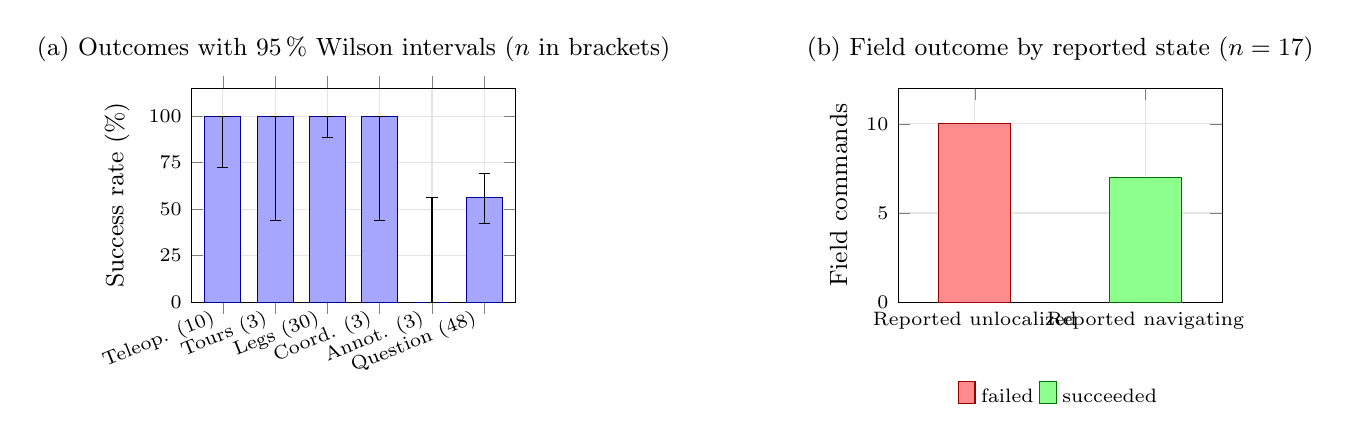
\begin{tikzpicture}
\begin{axis}[
  name=ax1, width=0.47\textwidth, height=4.3cm,
  ybar, bar width=13pt, ymin=0, ymax=115,
  ylabel={Success rate (\%)}, ylabel style={font=\small},
  symbolic x coords={Teleop.,Tours,Tour legs,Coord.,Annot.,Question},
  xtick=data,
  xticklabels={Teleop. (10),Tours (3),Legs (30),Coord. (3),Annot. (3),Question (48)},
  x tick label style={font=\scriptsize, rotate=22, anchor=east},
  ytick={0,25,50,75,100}, tick label style={font=\scriptsize},
  enlarge x limits=0.12, grid=major, grid style={gray!20},
  title={(a) Outcomes with 95\,\% Wilson intervals ($n$ in brackets)},
  title style={font=\small},
]
\addplot+[fill=blue!35, draw=blue!60!black,
  error bars/.cd, y dir=both, y explicit, error bar style={black}]
 table[x=k, y=v, y error minus=lo, y error plus=hi] {
k            v     lo    hi
Teleop.      100   27.8  0
Tours        100   56.2  0
{Tour legs}  100   11.4  0
Coord.       100   56.2  0
Annot.       0     0     56.2
Question     56.2  13.9  13.1
};
\end{axis}
\begin{axis}[
  at={(ax1.right of south east)}, xshift=1.5cm, anchor=left of south west,
  width=0.47\textwidth, height=4.3cm,
  ybar stacked, bar width=26pt, ymin=0, ymax=12,
  ylabel={Field commands}, ylabel style={font=\small},
  symbolic x coords={Reported unlocalized,Reported navigating},
  xtick=data, x tick label style={font=\scriptsize},
  tick label style={font=\scriptsize}, enlarge x limits=0.45,
  grid=major, grid style={gray!20},
  title={(b) Field outcome by reported state ($n=17$)}, title style={font=\small},
  legend style={font=\scriptsize, at={(0.5,-0.34)}, anchor=north, legend columns=2, draw=none},
]
\addplot+[fill=red!45, draw=red!60!black] coordinates {(Reported unlocalized,10) (Reported navigating,0)};
\addplot+[fill=green!45, draw=green!45!black] coordinates {(Reported unlocalized,0) (Reported navigating,7)};
\legend{failed, succeeded}
\end{axis}
\end{tikzpicture}
\caption{(a)~Measured outcomes. Intervals are wide because samples are small; the annotation
arm of the bench comparison and the coordinate arm do not separate at $p=0.10$. (b)~In the
field record, reported localization state separates success from failure perfectly, and the
addressing scheme does not separate them at all.}
\label{fig:results}
\end{figure*}

\subsection{System indicators}

Table~\ref{tab:metrics} collects the measured indicators. We report guided-tour completion at
two levels, because the 30 legs are not independent observations: a leg that fails ends the rest
of its tour. The leg-level interval is therefore optimistic, and the tour-level one is the
conservative reading.

\begin{table}[!t]
\caption{Measured indicators, June--July 2026. Legs within a tour are not independent
observations, so the leg-level interval is optimistic.}
\label{tab:metrics}
\centering
\scriptsize
\setlength{\tabcolsep}{3pt}
\begin{tabular}{@{}p{3.05cm}rp{1.55cm}p{1.55cm}@{}}
\toprule
\textbf{Indicator} & \textbf{$n$} & \textbf{Value} & \textbf{95\,\% interval} \\
\midrule
Teleoperation success            & 10 & \SI{100}{\percent} & \numrange{72.2}{100}\,\% \\
Guided tours completed           & 3  & \SI{100}{\percent} & \numrange{43.8}{100}\,\% \\
\quad individual legs            & 30 & \SI{100}{\percent} & \numrange{88.6}{100}\,\% \\
Tour duration (median)           & 3  & \SI{670}{\second}  & \numrange{668}{822}\,s \\
Coordinate goal, bench           & 3  & \SI{100}{\percent} & \numrange{43.8}{100}\,\% \\
Annotation goal, bare client     & 3  & \SI{0}{\percent}   & \numrange{0}{56.2}\,\% \\
Repeat-question match            & 48 & \SI{56.2}{\percent}& \numrange{42.3}{69.3}\,\% \\
Speech-bridge latency (mean)     & 5  & \SI{923}{\milli\second} & \numrange{651}{1555}\,ms \\
Local REST latency               & -- & $<\SI{100}{\milli\second}$ & -- \\
Wi-Fi round-trip time            & -- & --                 & \numrange{89}{1654}\,ms \\
\bottomrule
\end{tabular}
\end{table}

Two negative results deserve as much visibility as the positive ones. On a controlled set of 12
questions with four paraphrases each, question matching succeeded in 27 of 48 trials
(\SI{56.2}{\percent}). Most of the failures were near misses, where overlapping keywords routed
a question to a neighbouring entry, rather than cases where nothing matched at all. That pattern
argues for a wider synonym set or a semantic fallback, not for moving the threshold. Voice
round-trip time ($n=12$) ranged from \SI{979}{\milli\second} to \SI{23}{\second}. The
distribution is badly skewed and we do not quote a mean, which here would describe none of the
observations.

\subsection{Comparison with the vendor application}

Table~\ref{tab:compare} compares the two systems capability by capability. It is not a
controlled user study, and where both provide a function we make no claim about which does it
better. The lower block lists the areas where the vendor keeps a real advantage, most of which
follow from resources a laboratory does not have.

\begin{table}[!t]
\caption{Capability comparison with the vendor application}
\label{tab:compare}
\centering
\scriptsize
\begin{tabular}{@{}lcc@{}}
\toprule
\textbf{Capability} & \textbf{Vendor} & \textbf{This work} \\
\midrule
Teleoperation, guided tour              & yes & yes \\
Speech synthesis                        & yes & yes (IPC bridge) \\
Speech recognition                      & yes (cloud) & yes (on-device) \\
Face re-identification                  & yes & yes (on-device) \\
Question answering                      & yes (cloud) & yes (local) \\
Operates without Internet               & no  & yes \\
Inspectable and modifiable logic        & no  & yes \\
Self-hostable, no vendor account        & no  & yes \\
\midrule
Multi-floor navigation                  & yes & no \\
Fleet management console                & yes & no \\
Maintenance and updates under warranty  & yes & no \\
Recognition quality across languages    & yes & partial \\
\bottomrule
\end{tabular}
\end{table}

%==============================================================================
\section{Discussion}
\label{sec:discussion}
%==============================================================================

\subsection{What the study establishes}

The methodological lesson is that discovery and verification are two different problems, and on
a closed platform the second is much the harder. Recovering names is fairly mechanical:
introspection plus a decompiler produce a large candidate surface in a matter of days.
Establishing that any of those commands does something is where the time actually goes, because
the interface reports success in exactly the same way whether or not the machine moves. Our
field record puts this as starkly as we could have wished. The outcome was settled by a state
field, and not at all by the command variant we had spent weeks trying to tell apart.

From this follows a design rule, and the rule has a price. Pair every command with an
independent observation of its effect, and re-establish explicitly every precondition the vendor
application sets implicitly. That preparation sequence is what separates a working integration
from a bench script that reports success and moves nothing. It is also not free. We had a
standing complaint that the robot felt sluggish, and traced it to preparation steps being issued
unconditionally on every command, which added two round trips and a fixed delay even when
telemetry already confirmed the required state. Skipping them once the state is confirmed is the
same discipline read backwards: do not re-issue a command whose effect the telemetry is already
reporting.

\subsection{Generalization}

H1 should hold wherever the vendor's companion application is the primary control surface, since
that application has no choice but to speak the true protocol. H4 should hold on any platform
that places a safety or mode-arbitration layer between the message bus and the actuators, which
is the norm for commercial mobile bases. The rejection of H2 is specific to this manufacturer,
and another may well command over a broker; what carries across is the triangulation procedure
that settled the question in a single audit instead of weeks of intermittent failures. Concrete
names, gate semantics and naming conventions do not transfer at all, and have to be
rediscovered, which is what the pipeline is for. We have run the method on one platform. Whether
it transfers to a second vendor is a claim we would like to make and cannot yet support.

\subsection{Ethics and data protection}

The robot belongs to our institution and was studied for interoperability. We analysed the
vendor application in order to recover message schemas, not to extract or redistribute
proprietary assets, and we bypassed no licensing or protection mechanism. Staying
non-destructive was an ethical commitment and a practical one at the same time: it leaves the
warranty and the update path intact, and it avoids producing a firmware fork that nobody would
maintain.

Face re-identification processes biometric data, and that needed a separate judgement.
Pretrained embedding models differ in the provenance of their training data, and several widely
circulated conversions descend from a corpus that was withdrawn over consent concerns. We chose
a model whose provenance is documented, obtained through a checksum-verified chain, and we
record the trade-off here rather than presenting the choice as settled. Enrollment is never
automatic. A staff member initiates it in the presence of the person being enrolled, who is told
at that moment what is happening, and individual embeddings can be deleted afterwards from the
operator interface. Only embedding vectors leave the head. No image is stored or transmitted.

\subsection{Limitations}

The evaluation is where this work is weakest. Our samples are small and the intervals in
Table~\ref{tab:metrics} are wide to match; the bench comparison in particular cannot support a
claim of difference at $n=3$ per arm, and we do not make one. We never instrumented
session-level connection reliability, so we describe the reconnection mechanism instead of
quoting a figure we cannot stand behind. The vendor comparison covers capabilities, not measured
task performance. H1 was confirmed in one direction only: observed names do appear in the
application, but we did not establish that the application exercises every command the firmware
will accept, so the surface we recovered is a lower bound. Ten recorded wake events are too few
to estimate a false-trigger rate, and the face-matching threshold has not been calibrated for
several visitors enrolled at once. All of it comes from one robot, one map and one site.

%==============================================================================
\section{Conclusion}
%==============================================================================

We asked whether the command surface of a closed Android--\ros{} service robot can be recovered
without the manufacturer's help, and what evidence that recovery demands. The seven-phase,
triangulation-based pipeline produced a working surface on a commercial reception platform, and
carried an edge deployment that replaces the vendor cloud for teleoperation, navigation, speech
and visitor interaction. Static analysis of the vendor application proved a dependable source of
protocol names and of the preconditions nobody documents (H1). The exposed broker turned out to
be incapable of carrying commands at all (H2). Above everything else, the gap between transport
and execution (H4) governed the entire exercise: the addressing scheme we had expected to matter
(H3) explained none of our field outcomes, while the precondition state explained all of them.

The obvious next steps are to run the method against a second manufacturer, to replace our
capability table with a measured task comparison, to collect enough navigation trials for the
two arms to separate, and to ground a language-model planner in the primitives we validated
rather than leave it to rediscover the interface for itself.

%==============================================================================
\section*{Acknowledgment}
%==============================================================================

We thank our robotics laboratory for robot access and for support during field testing.

\bibliographystyle{IEEEtran}
\bibliography{references}

\end{document}
